\subsection{Arrays}

\Xten{} arrays provide support for the creation and manipulation of
distributed multi-dimensional arrays. Once created, any activity can
operate on arbitrary regions of the array, potentially through asyncs. The
implementation of \Xten{} arrays in \Xtenlib{} will provide the
interface for all \Xten{} array operations viz., point-wise, reduction,
scan. Also, an efficient iterator function will be provided. The maximum rank
(i.e. the number of dimensions) of the array supported by
the library will be fixed to a small constant (say 7). 

A distributed array consists of two key components -- meta-data and
data. The meta-data consists of information about the array, like,
shape (rank and size of each dimension), distribution etc. 
The meta-data is stored in the local heap of each process and
is immutable.
The data consists of the actual array data. The data is allocated
in the hosted address space of each process. The meta-data and
data are referred to as {\tt array\_info} structure.  

We categorize the distributed arrays into three kinds -- {\em regular},
{\em semi-regular} and {\em irregular}. The regular arrays are created
only by the root process (ie. the process that executes the first
activity) and have very regular distribution -- that is,
all the processes own a chunk of data and the chunks are of same size
in all the nodes. Semi-regular arrays satisfy the property that it can
be allocated by the root process; the other two properties of regular array
do not hold. Irregular arrays are the most
general arrays which don't have any of the above 3 constraints of the 
regular arrays. For efficiency in array access operations,
we plan to allocate each of these arrays differently.

\subsubsection{Regular Arrays}
\begin{figure}
\center
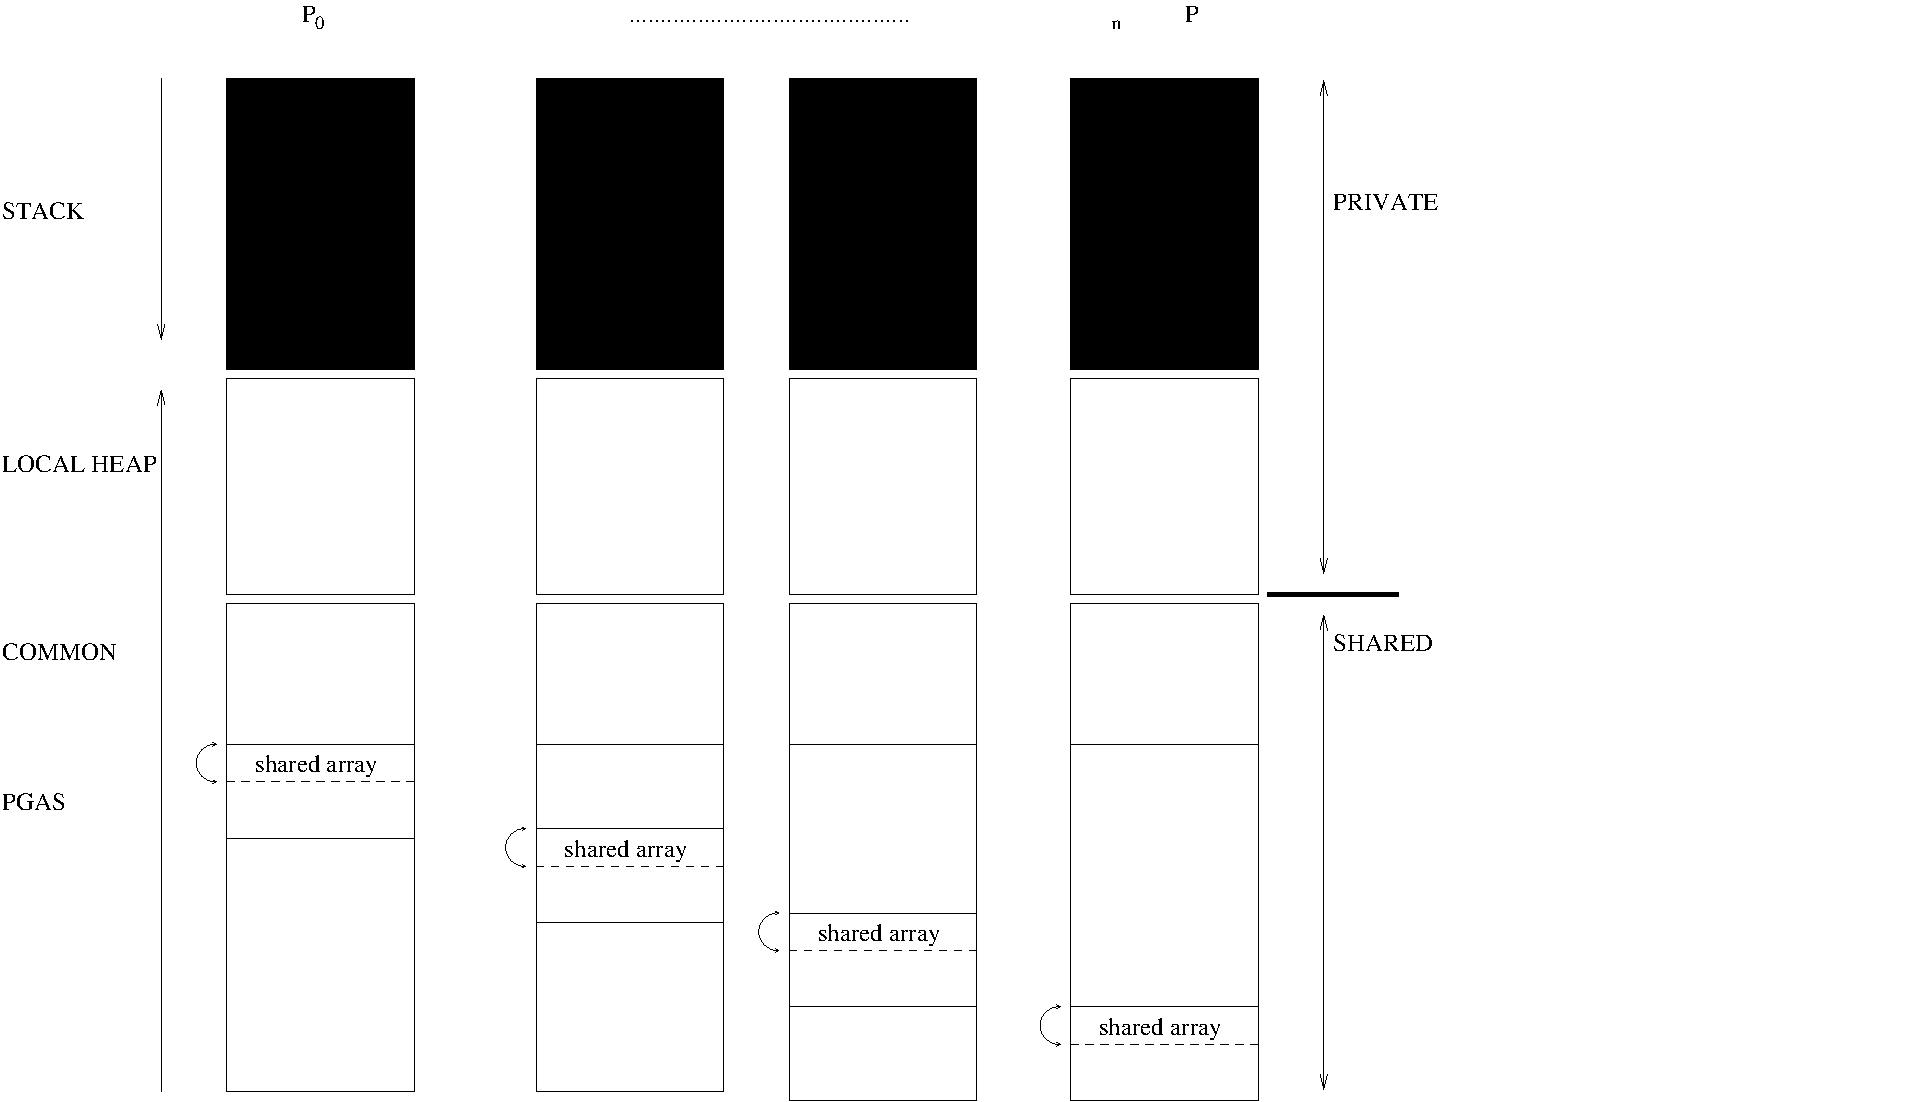
\includegraphics[scale=0.5]{ARRAY-REGULAR}
\caption{A sample layout of a {\em regular} distributed array}
\label{fig:array_layout_regular}
\end{figure}

For regular arrays, we plan to exploit the benefits of GAS and the compiler.
The chunks of regular arrays are allocated in a special region called {\em array}
region. This array region is a part of the PGAS. All the process allocate its
chunk in the same base address, with the first word containing a pointer to 
the meta-data. The rest of the words contain the data. This allocation scheme is shown in Figure~\ref{fig:array_layout_regular}.

The main advantage of this allocation is that an array access like $a[i]$ will
be directly compiled to the following target code by the compiler : $get(((a.base \& mask) | node\_id) + local\_offset(i))$.
Thus, no extra table lookup is required, unlike the allocation scheme that we will see in the following
sections.

Consider again the RandomAccess code of Section~\ref{sec:deploy:example}. The code
has two distributed arrays - {\tt table} and {\tt ranStarts}. Both these arrays
are created in the beginning of the program as follows:

\begin{verbatim}
1: final long[.] table = new long[block(TABLE_SIZE)] 
2:               (point p[i]) { return i; };
3: final long[.] ranStarts = new long[unique()]
4:		(point p[i]) { return C.starts(N_UPDATES_PER_PLACE*i); };
\end{verbatim}

The root process invokes the array constructor. The array constructor
determines the base address where the array needs to be allocated. It then
sends a message to all the processes to allocate the array at the same
base address in their section of PGAS along with initial data
and meta-data of the array. The processes receive the message,
allocate the array and initialize it. The array construction terminates only
after the message is received and the arrays are allocated and initialized
at the receiving end.

\subsubsection{Semi-regular Arrays}

\begin{figure}
\center
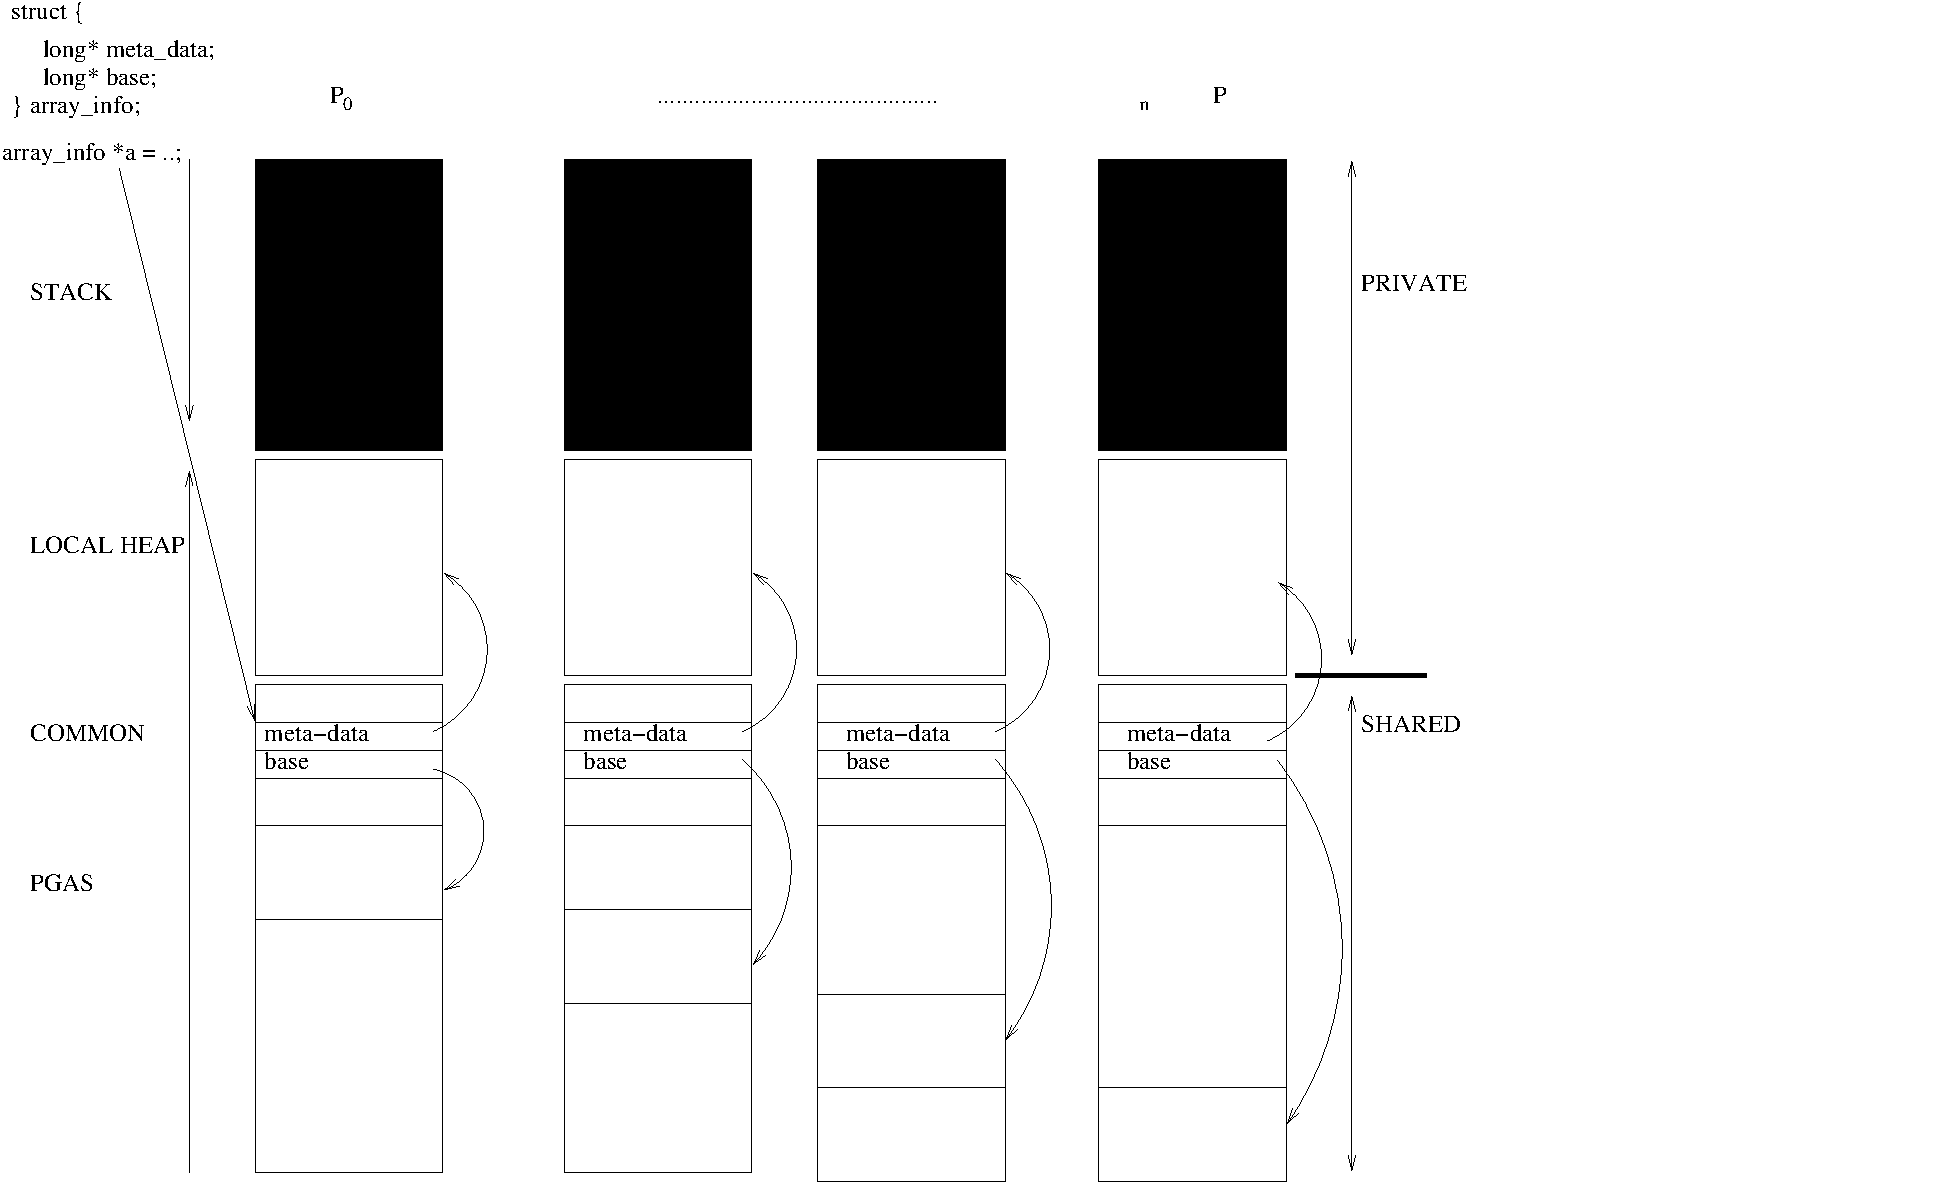
\includegraphics[scale=0.5]{ARRAY-SEMI}
\caption{A sample layout of a {\em semi-regular} distributed array}
\label{fig:array_layout_semiregular}
\end{figure}

For semi-regular arrays, the
{\tt array\_info} is stored in the common address space. The root process
sends a message to all the process to allocate the {\tt array\_info}
in the same address. Upon receiving this message, each processor
allocates the space for {\tt array\_info} (in the common address space), meta-data 
(in the local heap) and data (in the hosted space). A sample layout of a
distributed array in the address space is shown in the Figure~\ref{fig:array_layout_semiregular}.

For example, in the RandomAcess code listed in the previous section, the root process
invokes the array construction. The root process sends
a (LAPI) message to each process requesting a block of the array to be allocated
on that process and initialized. Initialization information and other information like the distribution are sent to the
processes in the message. 
Upon receiving the message, each process creates a meta-data for the array
in its local heap, and allocates a region in its hosted address space (cf. Section~\ref{sec:gas})
for the local data section of the array. It also stores the {\tt array\_info}
in the address sent by the root process in the common address space. 
The call to the array creation routine returns only after the message
is received by the processes involved, and the array sections are initialized
in each process. 

\subsubsection{Irregular Arrays}

\begin{figure}
\center
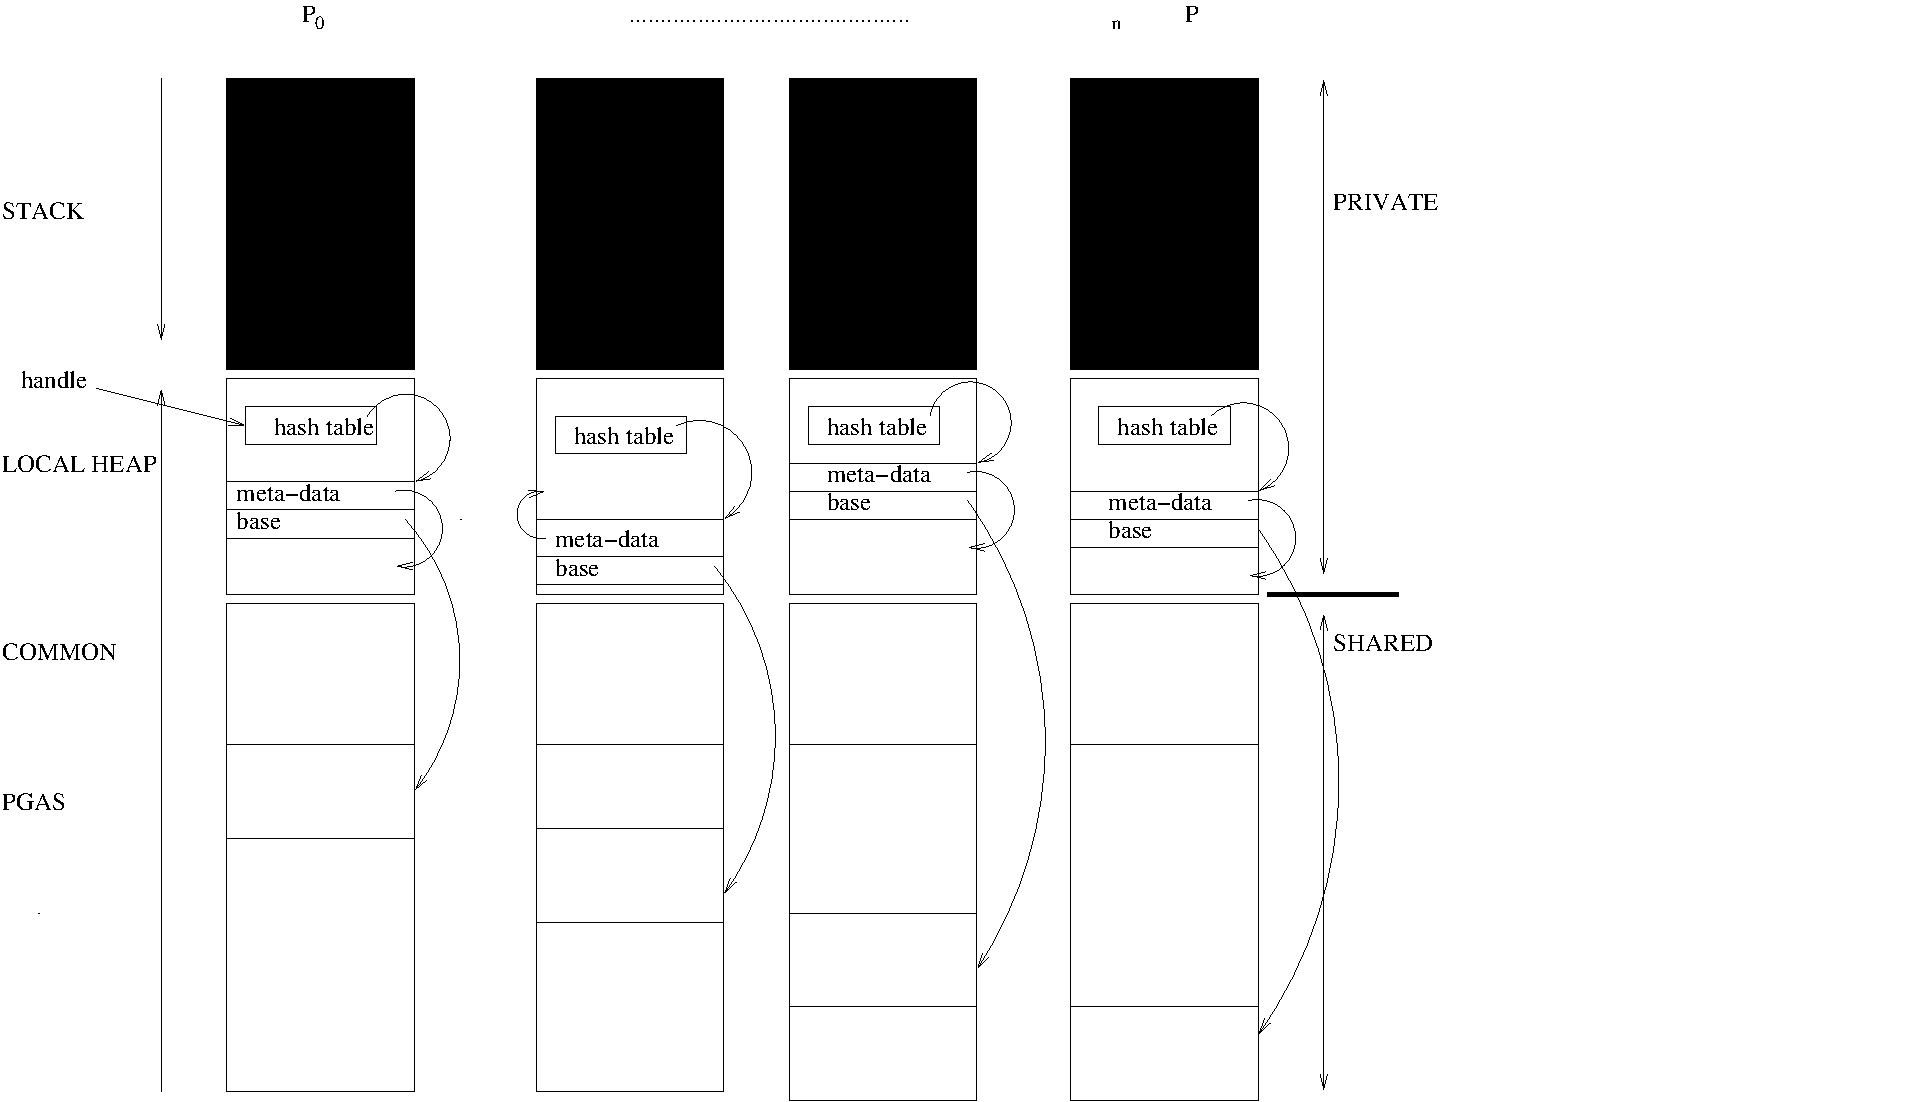
\includegraphics[scale=0.5]{ARRAY-IRREGULAR}
\caption{A sample layout of an {\em irregular} distributed array}
\label{fig:array_layout_irregular}
\end{figure}

Irregular arrays are the most general arrays. For these arrays, we generate
a unique handle to represent the distributed array. This unique handle
can be generated by the concatenation of process ID and a local counter.
(ie. $\langle$process id,local counter$\rangle$). A hash-table is allocated
in the local memory of each process. The unique handle is used to lookup in to
the hash table and obtain the {\tt array\_info} for the given handle (array). 
This scheme is shown in the Figure~\ref{fig:array_layout_irregular}.

For example, in the RandomAccess code, the activity that creates the 
arrays (not necessarily the root activity), constructs an unique handle
using the above mentioned scheme. It then sends this handle and other
information (initial values, meta-data etc.) to the other processes
that need to allocate a section of the distributed array. On the receiving 
end, each process allocates the {\tt array\_info} in its local memory.
The data for the array is allocated in their section of PGAS. The pointer
to the {\tt array\_info} is stored in the hash table entry corresponding
to the unique handle sent by the activity that invoked the array constructor. 

%In architectures such as BlueGene/L, without native support for RDMA,
%identifying the local buffer base address at the remote node is
%efficient. This is how the implementation of shared value directories
%is done in UPC on BlueGene/L~\cite{PLDI06}.  On architectures supporting
%zero-copy RDMA, \Xtenlib{} combines the above approach with a cache of
%shared array information on remote nodes on which they were recently
%accessed. Thus the first communication is expensive, being implemented
%by a remote activity, but subsequent remote memory access is through
%optimized put/get operations.

%Another design alternative is to choose the base address of the local section of the array to be
%same on all the nodes. This might involve an all-to-all communication among
%the nodes to decide the common base address. Since \Xtenlib{} provides the 
%global address space (GAS) abstraction (Section ~\ref{sec:gas}), choosing a common base address is a
%natural way to represent shared arrays.

%Prevalent runtime systems create shared arrays collectively.  Each
%process assign an index in a meta-data table for the shared array
%being created. Assuming all processes are involved in the shared array
%creation and they do so in the same order, all processes can decide on
%the same entry index in the local meta-data tables. This index is used
%as the globally unique handle.

%\Xtenlib, supporting the non-collective shared array creation, uses a
%$\langle$place id,local counter$\rangle$ from the creating activity as
%the shared array handle. Unlike in typical implementations in which
%the shared arrays handles index into a table, they index into a hash
%table.
